%!TEX root = ../Masterarbeit.tex
\chapter{Konzeption}
\label{cha:konzeption}
Im Folgenden wird das Konzept der Web-Applikation erarbeitet und vorgestellt. Dafür wird vorerst ein Fernkonzept und ein dazugehöriges Mockup erstellt, wobei das Fernkonzept über den gesamten wünschenswerten Umfang einer solchen Applikation verfügen soll.  Das bedeutet, dass die Applikation nicht auf mögliche Medieninhalte und -typen beschränkt werden soll, sondern den heute und in naher Zukunft möglichen Spielraum ausnutzen soll.
Auf dieser Basis wird ein Mockup der im weiteren Verlauf bei ihrem Arbeitstitel \textbf{\arbeitstitel} benannten Web-Applikation entwickelt, welches die Anwendungsfälle und Darstellungsmöglichkeiten beinhaltet.
Anschließend wird das Fernkonzept auf ein im Rahmen dieser Masterarbeit realisierbaren Umfang reduziert und entsprechend eingegrenzt. Am zuvor erstellten Mockup sollten diesbezüglich nur wenige Änderungen \bzw Einschränkungen vorgenommen werden müssen.

%===== SECTION =====%
\section{Anforderungsanalyse}
Aus der vorangegangenen Analyse der vorhandenen Suchdienste geht hervor, dass es eine umfassende Suche nach zeitspezifischen Inhalten bisher nicht sehr komfortabel ist, \bzw nicht immer relevante Suchergebnisse liefert. Diese Möglichkeit soll die Web-Applikation, die im Rahmen dieser Arbeit entwickelt wird, bieten. Über welche Funktionalität sie im Konkreten verfügen soll, wird im Folgenden analysiert und anschließend in einer Feature-Liste aufgeschlüsselt.

\subsection{Eingabeformen}
Ausgangspunkt für die Suche ist ihre Eingabeform. Der Nutzer soll hinsichtlich der Art seiner Eingabe möglichst frei sein können. Über die Text-Suche, wie sie in der vorangegangenen Analyse (siehe \ref{sec:suchdienste}) durchgeführt wurde, gibt es noch weitere denkbare Möglichkeiten.

\paragraph{Datum}
Die Eingabe eines Datums ist die naheliegendste Suchform um Kontent, der sich auf einen Zeitpunkt \bzw dessen umschließenden Zeitraum bezieht.

\paragraph{Ereignis, Zeitraum oder Epoche}
Primär sind Begriffe wie \zB \glqq 1937\grqq \ oder \glqq 12.04.1922\grqq \ denkbar. Darüber hinaus lassen sich viele Begriffe auch in Zeiträume oder Zeitpunkte aufschlüsseln, wie \zB die Begriffe \glqq Neunziger\grqq , \glqq Vietnamkrieg \grqq oder \glqq Deutscher Mauerfall\grqq . 

\paragraph{Musik oder Film}
Aus einer Musik- oder Film-Veröffentlichung kann ebenfalls ein Datum entnommen werden. Hier bietet sich beispielsweise das Veröffentlichungsdatum oder das Produzierungsdatum an, während bei einer TV-Produktion die Erstausstrahlung und bei einem Kinofilm der Filmstart relevant ist.

\paragraph{Bild oder Kunst}
Im Falle von Bild oder Kunstwerken ist die Zuhilfenahme der Aufnahmedatums oder die Fertigstellung eines Kunstwerkes denkbar. Viele Kunstwerke \oae \ der frühen Vergangenheit lassen sich auf keinen genauen Zeitpunkt zurückdatieren, oftmals existiert in diesen Fällen ein möglicher Zeitraum, in welchen es fertig gestellt wurde.

\paragraph{Personen}
Auch anhand einer Person kann ein Zeitraum ermittelt werden. Dies kann je nach Interesse der gesamte Lebenszeitraum sein oder auch ein Zeitraum, in dem diese Person von größerer Wichtigkeit war (Amtsperiode, Aktivitätszeitraum eines Musikers).

%----- SUBSECTION -----%
\subsection{Funktionen}
Die Kernfunktionalität der Web-Applikation ist die Suche nach Inhalten, die aus einem spezifischen Zeitraum stammen, \bzw sich mit diesem Zeitraum befassen. Darüber hinaus soll der Inhalt auf unterschiedliche Weise präsentiert werden und konsumiert werden können. Hauptsächlich soll eine visuell ansprechende Form der Inhalte präsentiert werden, gleichzeitig soll es dem Nutzer ermöglicht werden, direkt in der Web-Anwendung Audio-Inhalte zu hören, während er sich weitere Ergebnisse seiner Suche ansieht. Ebenso soll es möglich sein, während des Durchstöberns der Suchergebnisse Video-Inhalte betrachten zu können.

%----- SUBSECTION -----%
\subsection{Kontent-Typen}
Anhand eines Zeitpunktes oder -raumes lassen sich eine Vielzahl unterschiedlicher Inhaltstypen anzeigen. Da es das Ziel der Web-Applikation ist, ein möglichst umfassendes Bild eines Zeitraumes anhand verschiedener Medien zu präsentieren, werden im Folgenden denkbare Inhalts-Typen erläutert.

\paragraph{Politische und geschichtliche Ereignisse}
Ein wichtiger Aspekt, der einen Zeitraum prägt, sind die darin auftretenden Ereignisse. Zum einen sind da politische Ereignisse wie \zB der Independence Day der USA, der Mauerfall, die Terroranschläge aber auch zeitprägende Begriffe wie die Goldenen Zwanziger, die Industrialisierung oder die Weltwirtschaftskrise. Ebenso gehören Natur-Ereignisse, als auch Medien-Ereignisse dazu. Hier kann als Beispiel die erste Landung eines Menschen auf dem Mond genannt werden. Ebenso interessant sind Informationen wie die Regierungsform oder die Parlamentszusammensetzung.

\paragraph{Demografische Daten}
Demografische Daten geben ebenfalls Aufschluss über einen Zeitraum. Die Zusammensetzung der Bevölkerung, ihre Dichte oder \zB das durchschnittliche Alter der Menschen sind Aspekte, die einen Zeitraum mit ausmachen. Genauso können Arbeitslosenquoten die Zufriedenheit der Bürger wiederspiegeln.

Darüber hinaus können Informationen über das vorherrschende Wetter von Interesse sein oder Informationen über die Länge des Tages.

\paragraph{Musik}
Musik repräsentiert einen großen Teil des kulturellen Aspekts eines Zeitraums. Musik aus einem bestimmten Zeitraum spiegelt nicht nur den Geschmack, sondern auch politische Neigungen oder beschäftigt sich mit aktuellen Themen, denkt man an den Song \textbf{Only Time}, der im Zuge der Terroranschläge vom 11. September an großer Popularität gewann. Dazu macht sie einen Teil des vorherrschenden Stils aus.

\paragraph{Kunst}
Verschiedenste Arten von Kunst haben schon die frühesten Epochen der Menschheit geprägt. Ähnlich wie die Musik spiegeln Kunstwerke ihrer Zeit nicht nur den Stil, sondern auch die aktuelle Situation, Wünsche, Träume und Bedürfnisse der Künstler und ihrer Zeitgenossen.

\paragraph{Film}
Film ist zwar im Gegensatz zu Kunst ein eher neues Medium, doch auch die Unterhaltungskunst des Films repräsentieren den Geschmack und Zeitgeist der Gesellschaft. Hinzu kann ein Film, der sich mit der Thematik aus der Vergangenheit beschäftigt im Nachhinein interessant oder gar wichtig sein. Darüber hinaus geben besonders neue Filmproduktionen ein Bild der Generationen wieder. So kann \zB der Film \textbf{Breakfast Club (1985)} einen Querschnitt derzeitiger Schüler geben und der Film \textbf{Back to the Future (1985)} eine, wenn auch nicht ganz ernstgemeinte, Annahme der Zukunft wiederspiegeln. \todo{raus?}

Hinzu kommen Video-Reportagen und -Berichte, die einen Zeitraum näher betrachten und selbst ein Bild eines Zeitraumes oder Ereignisses darstellen. Sonstiges Video-Material, wie \zB Filmtrailer lassen sich auch in diese Kategorie zählen.

\paragraph{Erfindungen und technische Errungenschaften}
Erfindungen haben bereits in der Vergangenheit großen Einfluss auf die Veränderung der Gesellschaft ausgeübt. Nicht nur die Erfindung des Buchdrucks, des Computers oder des Internets haben zu ihrer Zeit und darüber hinaus das Leben der Menschen verändert. Ebenso interessant können zeitnahe Reaktionen und Annahmen zu solchen Erfindungen sein, geben sie \uU Aufschluss über die Haltung der Menschen gegenüber der Fortschritte. So \zB die frühe Annahme, dass Geschwindigkeiten von über 30 km/h dem menschlichen Körper tödlich schadeten.

\paragraph{Video-Spiele}
Im fortgeschrittenen Zeitalter ist auch eine Darstellung von Video-Spielen, die zu der Zeit erschienen sind. Sie geben ebenfalls Aufschluss über die derzeitigen technischen Möglichkeiten.

%----- SUBSECTION -----%
\subsection{Darstellung}
Bei einer Darstellung so vieler verschiedener Arten von Daten, muss das Layout sowohl variabel, als auch konsistent sein. Die Breite der Inhalte kann sich sehr oft verändern, wenn neue Quellen hinzugefügt werden und eine bestimmte Darstellungsform erfordern. Gleichzeitig darf das Layout durch die Masse an unterschiedlichem Inhalt nicht an Übersichtlichkeit und Konformität einbüßen.

Inhaltstypen müssen für den Benutzer klar erkennbar sein, sodass Audio-Daten schnell von Text-Daten \oae unterschieden werden könnnen. Außerdem soll der Nutzer komfortabel und unkompliziert durch die Ergebnisse navigieren können.


%===== SECTION =====%
\section{Features}
%----- SUBSECTION -----%
\subsection{Eingrenzen der Suche}
\begin{itemize}
	\item Medientypen (Audio, Video, Text, Tabellen, Diagramme)
	\item Quellen(APIs, Suchdienste, etc.)
\end{itemize}

\subsection{Filtern des Ergebnisses}
\begin{itemize}
	\item Kategorien (Stil, Genre)
\end{itemize}

%----- SUBSECTION -----%
\subsection{Thematisches Suchen}
Während die Suche nach einem bloßen Datum stringent alle auffindbaren Informationen, die in diesen Zeitraum fallen, anzeigt, muss es auch möglich sein, gezielt thematisch zu suchen. Zum Beispiel soll es die Möglichkeit geben ausschließlich Daten eines Zeitraumes, die sich auf das Thema Musik beziehen. Dabei sind keinesfalls lediglich Musikdateien gemeint, sondern auch \bspw Text- oder Videoquellen, die sich mit dem Thema Musik beschäftigen. Das Ergebnis wäre ein Bild der derzeitigen Musikgeschichte zu bekommen.

%----- SUBSECTION -----%
\subsection{Inhaltseingrenzung}
Um den Nutzen der Web-Applikation möglichst vielseitig zu halten, kann bei der Suche die Art des Inhalts eingegrenzt werden. So kann die Wahl getroffen werden, welche Medientypen angezeigt werden sollen (Audio, Video, Text etc.). Auch ist eine Filterung der in Betracht gezogenen Dienste denkbar, sodass der Nutzer \bspw bestimmte APIs deaktivieren kann.

%\subsection{Filtern}
%----- SUBSECTION -----%
\subsection{Betrachten von Inhalten}

%==============================================================================%
%==============================================================================%
%==============================================================================%
%==============================================================================%
%==============================================================================%
%==============================================================================%

%\section{Funktionen}

\begin{figure}[htb]
	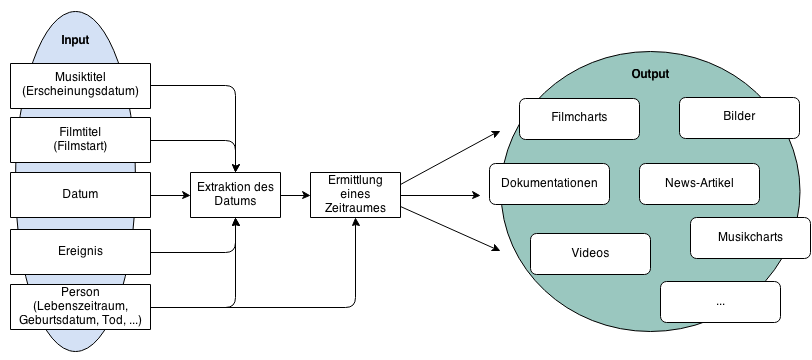
\includegraphics[width=1.0\textwidth]{Diagramm_Allgemein.png}
	\caption{Allgemeines Diagramm}
	\label{fig:diagrammAllgemein}
\end{figure}

\begin{figure}[htb]
	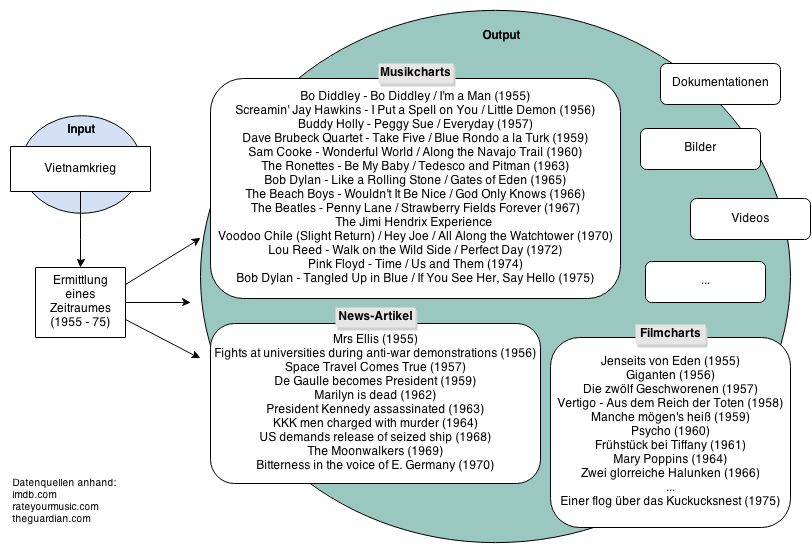
\includegraphics[width=1.0\textwidth]{Diagramm_VietnamKrieg.png}
	\caption{Vietnam Diagramm}
	\label{fig:diagrammVietnam}
\end{figure}

%Diagramm_VietnamKrieg.png

%===== SECTION =====%
\section{Fernkonzept}

Zunächst werden die Schlüsselaspekte, die in die Konzeption einfließen, erläutert.

%----- SUBSECTION -----%
\subsection{Inhalte}

\begin{itemize}
	\item Suche-Restriktion
	\item Suche Filter
	\item Suche Verfeinerung
\end{itemize}

%----- SUBSECTION -----%
\subsection{Suchefilter}
Mit der Grundeinstellung wird der Zeitpunkt als Zeitraum durchsucht. \Dahe dass vom Zeitpunkt ausgehend nach Medien in der nahen Vergangenheit als auch der Zukunft gesucht wird. Außerdem kann der Zeitraum, in dem gesucht wird, eingegrenzt werden. Zum einen kann vom Zeitpunkt ausgehend gesucht werden. Darüber hinaus kann die Suche so begrenzt werden, dass nur zu dem Zeitpunkt vorhandene Daten angezeigt werden.

Außerdem kann die Suche nach Thema eingegrenzt werden. Denkbar sind hier Themen wie Musik, Politik, Kunstgeschichte \ua Dies beinhaltet trotzdem sämtliche Medientypen, mit der Restriktion, dass der Content sich auf das Thema bezieht. Beispielsweise kann dies Videomaterial einer politischen Rede, die in dem Zeitraum stattgefunden hat oder ein Zeitungsartikel, der sich mit einem bestimmten Musiktitel auseinandersetzt.

Darüber hinaus gilt es Content aus der Zeit von Content über diese Zeit zu unterscheiden. Auch hier besteht die Möglichkeit das Ergebnis einzugrenzen.

\paragraph{Ort}
Die Suche kann spezialisiert werden, indem die Suchanfrage verfeinert wird. Das kann er zum Beispiel mit der zusätzlichen Angabe eines Ortes machen. Hier würden \zB Musik-Charts des jeweiligen Landes durchsucht und demografische Daten angezeigt.

\paragraph{Genre}
Insbesondere bei Audiodaten finden sich in den ID3-Tags Informationen über das Genre des Musikstückes. Konnten mehrere Genres ausgemacht


%----- SUBSECTION -----%
\subsection{Ergebnis-Filter --- Sortieren}
Sortieren

\begin{itemize}
	\item Relevanz
	\item Datum (nur wenn Daten ausgehend von einem Zeitpunkt in die Zukunft ODER der Vergangenheit angezeigt werden?)
\end{itemize}

Darüber hinaus kann das Suchergebnis nach Medientypen gefiltert werden. Möchte sich der Nutzer beispielsweise nur einen Radiosender generieren lassen und wünscht keinen Video-Content, kann der Nutzer das Ergebnis eingrenzen.

%----- SUBSECTION -----%
\subsection{Suchmöglichkeiten}
Der Nutzer soll in der Art, in der er suchen kann, möglichst frei agieren können. Jedoch muss es Restriktionen geben, die Suchbegriffe und das jeweilige Ergebnis der Suche verbessern.

Im Fokus der Applikation steht der Zeitpunkt, der dargestellt werden soll. Dementsprechend soll es dem Nutzer möglichst offen stehen, wie er seine Suche formuliert, solange der Suchbegriff sich in einen Zeitpunkt auflösen lässt.


Zeitpunkt <--

%===== SECTION =====%
\section{Mockup}

%----- SUBSECTION -----%
\subsection{Funktionalität}
Fokus der Applikation ist eine komfortable Suche, die dem Nutzer möglichst einfach zugänglich gemacht wird, \dahe vom Design, als auch von der Funktionalität. 
Eine für diese Web-Applikation besondere Aufgabe ist es, die drei Kernfunktionen möglichst gleichzeitig gut erreichbar zu machen, ohne die Gesamterscheinung zu stören.
\paragraph{Suchen}

\paragraph{Browsen}

\paragraph{Konsumieren}
Unter den dargestellten Inhalten befinden sich auch abspielbare Inhalte. Diese soll der Nutzer sich möglichst gleichzeitig anschauen können


Fokus der Applikation ist eine komfortable Suche, anhand dessen der Nutzer keine falschen Vorstellungen über die gelieferten Ergebnisse bekommt. \todo{doofer Satz, aber vielleicht nur die falsche Stelle}

%----- SUBSECTION -----%
\subsection{Design und Layout}
Da die Web-Applikation sehr viele unterschiedliche Medienarten und -inhalte darstellen soll, ist ein sauberes aufgeräumtes Design umso wichtiger, um es dem Nutzer zu ermöglichen, sich auf die Inhalte zu konzentrieren. Darum ist es wichtig, dass das Design möglichst wandelbar ist, unabhängig vom Inhalt. Folgende Aspekte sind beim Layout zu beachten:

\paragraph{Suche und Filter}

\paragraph{Musik-Player}

\paragraph{Video-Player}


%===== SECTION =====%
\section{Eingrenzung}